This section will describe the wireless communication and machine learning concepts involved in this work at a high level. The section starts with wireless channels, channel sounding and channel reconstruction. Then the section provides background to the algorithms used for channel reconstruction: LASSO, YOLO, and DNNs.  

\subsection{Wireless Concepts}
The wireless channel is the physical medium traversed by the signal. The channel is described mathematically by a matrix of complex numbers, H. The received signal \(\textbf{Y}\), is related to the transmitted signal as follows, \(\textbf{Y} = \textbf{H} \textbf{S} + \textbf{Z} \). Where \(\textbf{S}\) is the transmitted signal and \(\textbf{Z}\) is additive white gausian noise. The goal of this work is to reconstruct the channel matrix \(\textbf{H}\), from the received signal \(\textbf{Y}\). The remainder of this subsection will define key concepts: channel sounding, channel reconstruction from paths, channel reciprocity, and channel sparsity.
\subsubsection{Channel Sounding}
Radio systems require knowledge of the channel they will be transmitting over to optimize the communication. Important decisions are made with this information, such as the modulation scheme or the beamforming precoding matrix. For instance, lower SNR channels can support more bits per symbol, increasing the channel's throughput. However, if the channel cannot support the modulation scheme chosen then the bit error rate will be so high that the signal cannot be recovered. Channel sounding is done by transmitting a reference signal over the channel. The reference signal contains pilot symbols known to both the transmitter and the receiver. The receiver uses the difference between the received signal and the expected signal to estimate the channel conditions. Using these estimates the system will calculate CSI metrics such as the Channel Quality Indicator (CQI), Received Signal Strength Indicator (RSSI), Precoding Matrix Indicator (PMI), and Rank Indicator (RI) \cite{Dahlman2018}. CQI is an integer index into a list of Signal to Noise Ratio (SNR); there are 15 values, the higher the CQI, the better the SNR. RSSI simply returns the signal power measured at the receiver in negative dB, it typically ranges from 0-127. PMI is used in MIMO systems, it is an integer index into a list of potential precoding matrices. The matrix selected will be multiplied by the signals to be transmitted, mapping and scaling them for the appropriate antennas. Figure \ref{fig:pmibook} is an example of a simple PMI codebook. This code book is for two transmit antennas, with either one or two layers. Layer in this context is the number of symbols being transmitted at once. Rank Indicator (RI) is related to the rank of the channel matrix, if the RI is one then there is one independent path between transmitting antennas and receiving antennas. Therefore, the transmission is limited to being one layer. RI operates as the maximum number of supported layers. The highlighted square in figure \ref{fig:pmibook} is the precoder matrix for a PMI of 1 and a system configured to transmit 2 layers.

\begin{figure}[H]
    \centering
    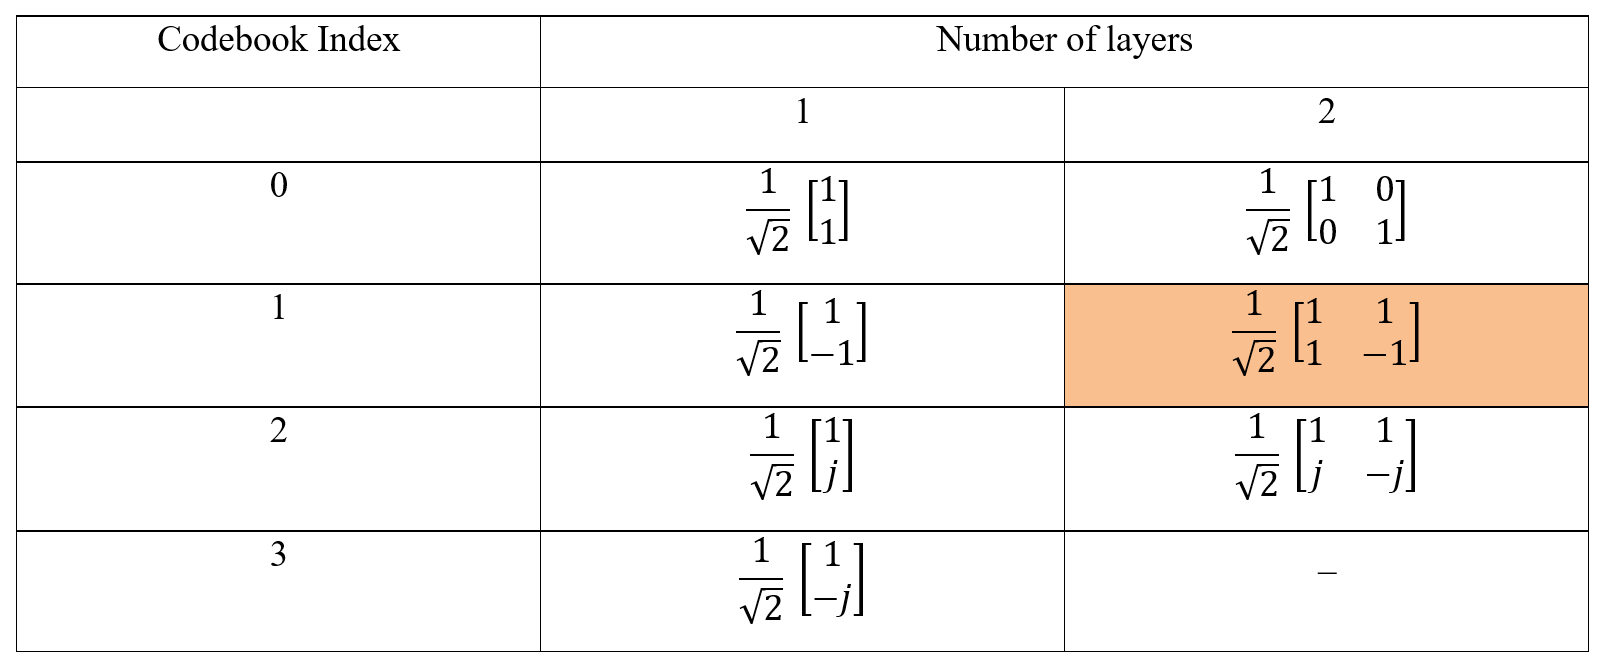
\includegraphics[width=15cm]{figures/PMI_Codebook.png}
    \caption{Example PMI Codebook \cite{Ryu2020}}
    \label{fig:pmibook}
\end{figure}

\subsubsection{Channel Reconstruction from Path Components} \label{sssec:chrec}

Wireless signals are impacted by objects in their path, causing them to experience reflection, refraction, and dispersion. Shadowing is the attenuation caused by obstacles in the path between the transmitter and receiver. Signals are not limited to following a single path to the receiver; often referred to as multipath effects. Each path will experience a different channel, as they may have different obstacles or distance. This will cause the signals to take a different amount of time to propagate to the receiver resulting in a different delay, phase, and gain for each of these paths. When adding signals that are out of phase they can either add constructively or destructively. Moving the receiver slightly can change the relative phase between signals causing a significant change in received power. Using knowledge of the path gains, angles, and delays the channel matrix can be reconstructed. The work done in \cite{Li2020} and \cite{Han2019} shows that the channel matrix is modeled with the following set of equations.
\[
    \textbf{h} = \sum_{l=0}^{L-1} g_{l} ( \textbf{p}_{l} (\tau) \otimes \textbf{a}(\theta_{l}) )
\]

\[
    \textbf{p}(\tau) = [e^{-j 2 \pi \frac{N}{2} \Delta f \tau}, ..., e^{-j 2 \pi (\frac{N}{2} - 1) \Delta f \tau}]
\]

\[
    \textbf{a}(\theta) = [e^{-j 2 \pi \frac{M}{2} \frac{d}{\lambda} \mathrm{sin}\theta}, ..., e^{-j 2 \pi (\frac{M}{2} - 1) \frac{d}{\lambda} \mathrm{sin}\theta}]
\]

\noindent
Note that \([\cdot]^{H}\) is the Hermitian Transform (complex conjugate transpose) and \(\otimes\) is the Kronecker Product. L is the number of paths. The individual path parameters \(g_l\), \(\tau_l\), and \(\theta_l\) are the gain, delay, and angle of the \(l^{th}\) path, respectively. Furthermore, \(\textbf{p}(\tau)\)and \textbf{a}\((\theta)\) are the delay-related phase vector and steering vector of a Uniform Linear Array (ULA) of antennas, respectively. All the remaining variables are constants chosen for a given communication system; \(d\) is the distance between antennas, \(\lambda\) is the carrier wavelength, and \(\Delta f\) is the carrier sub-spacing. This set of equations will be used to reconstruct the channel matrix after predicting the path components.

\subsubsection{Channel Reciprocity}
One of the main advantages to Time Division Duplexing (TDD) is that the uplink and downlink channels are the same; this is known as channel reciprocity. Alternatively, Frequency Division Duplexing (FDD) channels will experience frequency specific channel effects. This requires FDD systems to do channel sounding in both the uplink and downlink directions, then feed the results back over the channel. TDD can skip the channel sounding feedback step since it knows the channel is the same etiher way. This feedback step has very high overhead, especially in m-MIMO systems. The previously mention channel reconstruction technique is advantageous because the all the path parameters are frequency independent with the exception of the gain. This means the uplink and downlink values will be the same, even in an FDD system. Therefore, using this channel reconstruction scheme, the only feedback needed is to tune the path gains \cite{Han2019}. 

\subsubsection{Channel Sparsity}
In FDD m-MIMO systems the concept of channel sparsity is quite important and is exploited in many channel sounding techniques, such as LASSO and Netwonized Orthogonal Matching Pursuit (NOMP). Sparsity simplifies the problem of finding a channel's characteristics. In the context of this report, channel sparsity is the spatial channel sparsity for a channel vector and assumes there is a finite number of paths for downlink communication between a Base-Station (BS) and it's User Equipment (UE). Channel sparsity exists due the local scattering effects at the BS's antennas, and the temporal and spatial limitations of the signal paths available for a particular user time due to factors like interference \cite{Liu2016}. As the number of antennas in our m-MIMO system increases the scattering effect is amplified and the available paths for a UE becomes more limited. Therefore, the desired channel vector can be estimated using techniques that take advantage of the sparse channel vector structure.

\subsection{Deep Neural Networks}

Deep Neural Networks (DNN) play an important role in our project as one of the project objectives was to explore deep learning methods for downlink channel reconstruction for m-MIMO systems.  DNN and deep learning involve using multi-layered neural networks using several different techniques, such as Convolution Neural Networks (CNN), skip connections, and residual neural networks \cite{Burkov2019}. The number of layers for a deep learning network can vary, but generally contains more than one hidden layer.
Convolution Neural Networks are machine learning models which contain convolution layers. Convolution layers consist of weighted filters that are applied over a large input matrix which usually originated from a image or video source \cite{Burkov2019}. CNNs were invented for image and video processing with applications of object detection and classification in mind. CNNs have important roots in problem areas such as autonomous vehicles. In our project, CNNs were employed in YOLO's object detection, more in the subsequent subsection.

\subsection{YOLO}

You Only Look Once (YOLO) are a series of real-time object detection models developed for coloured images with complex classification targets. With real-time requirements for video detection, the model is very quick due to the fact that an image is processed with one pass of the deep network \cite{Redmon2018}. YOLO works differently than other object detectors which use classifiers or localizers to locate potential targets within an image and then run the model over different section of the image at three different scales. Running the detection process at three different scales enables YOLO to also detect objects that are of smaller size in an image, making it an ideal candidate for the detection of the small path objects discussed in Section \ref{image-gen}. YOLO passes the whole image through the detection model giving it an advantage of run-time speed and also the ability to take into account the global context of the whole image. YOLO's network structure can be split into three parts for the proposes of the report; the input layer, the hidden layers, and the output layers.

The input layer of YOLO takes a compressed version of an image to run detection over before delivery to the first CNN in the hidden layers. Compression of the image is very common in deep learning in order to lower the complexity of the model and also improve training and run-time. The input layer specifies three values which define the required image input size. The parameters are image width, height, and number of channels. Width and height describe the image size while the number of channels represent the values for each pixel. A grayscale image will have only one channel while a common RGB image has three channels. YOLO's pretrained models available for transfer learning use three channels to process RGB images, so any grayscale images must be preprocessed before the YOLO model can be used.

The hidden layer of YOLO changes depending on the version of YOLO in use. YOLOv2 uses Darknet-19, while YOLOv3 uses Darknet-52 \cite{Redmon2018}. The exact YOLO hidden network architecture can be substituted though with other network structures that preform well in objection detection such as ResNet-50 \cite{Matlab2021a}. The hidden layer provides the backbone for the object detection network and is where most of the training of our model's weights will occur. Darknet is an open-source neural network framework written for deep neural network design. As mentioned above, Darknet was used in the construction of both YOLOv2 and YOLOv3 and their training. Having the flexibility to change the network structure is quite important so that the network can adapt to the specific application. This flexibility also enables the construction of networks with varying hidden layer designs. In the case of our project, we did not need to take advantage of all 53 convolution layers of Darknet-53 because we believe the images that we are processing are much more simple than a complex RGB image with many different shapes and objects within the image. The images produced only have one class and has an object shape that is quite consistent making picking up the object with the CNN much easier. More on this in Section \ref{yolo-main} when model tuning is discussed.

The last part of the YOLO model are the output layers. For the process of object detection to be complete the output from the last or one of the convolution layers is taken and transformed into a series of anchor boxes that are uniformly distributed across the image data. These boxes represent the regions of interest in the image and each box predicts the probability of a target object lying within. The transform layer connects the output of the chosen convolution layer and the final output layer and evaluates the initial anchor boxes. The final output layer refines the predictions and anchor boxes from the previous transform layer producing the final output \cite{Matlab2021a}. 

When the three parts of the YOLO network model are combined, a preprocessed image can be given to the model to predict the location and bounds of target objects within the image. A threshold is used to determine which anchor boxes of the detector are valid and which are false positives. Therefore the threshold can be viewed as a hyperparameter for tuning the network detection of objects within the image. It is especially handy for our project's application since there is only one class of object of interest. This means that the threshold can be lower than normal to ensure all channel paths within an image are gathered. By default the threshold of object detection models in MATLAB is 0.5, but can be easily modified for different applications.

\subsection{LASSO} \label{lasso-back}

Least Absolute Shrinkage and Selection Operator (LASSO) is a linear regression technique that shrinks the absolute prediction error and is accompanied with a tuning parameter $\lambda$ which defines the minimum value of the sum of the regression coefficients \cite{Ranstam2018}. LASSO is a type of L1 regularization method since it contains an added penalty parameter to reduce the number of coefficients within the weights \cite{Ranstam2018,Tibshirani2013}. This type of regularization can be very useful for activities such as feature selection and models that have sparse structures such as the channel sparsity in FDD m-MIMO systems. LASSO can be represented mathematically using the following definition:

\[ \min_{\beta} \norm{y - x\beta}^2_2 + \lambda |\beta|_1 \]

Where \(y \in \mathbb{R}^{M \times 1}\),  \(x \in \mathbb{R}^{M \times N}\), \(\beta \in \mathbb{R}^{N \times 1}\), and \( { \lambda \in \mathbb{R} | \lambda \geq 0 } \). $x$ defines our $M \times N$ input matrix and $\beta$ are the unknown coefficients applied to the matrix to generate the output vector $y$. LASSO regression will minimize or eliminate the coefficients in the $\beta$ vector to satisfy the equation above. Setting $\lambda = 0 $ will just perform normal linear regression as the penalty proportion would go to zero. Increasing the value of $\lambda$ will increase the sparsity of the $\beta$ vector by setting more and more of the values in $\beta$ to zero.

As described in the paragraph above, the LASSO regression functions on real valued matrices and vectors whereas in the application of channel reconstruction, the values used to represent the channel vector and signals are complex values ($H,x,y \in \mathbb{C}$, where H, x, and y are the channel vector, transmitted signal, and received signal respectively) \cite{Liu2016}. To overcome this complication, the normal LASSO regression function defined in MATLAB has to be modified or another LASSO function has to be imported to handle the complex values of the channel model's representation. Both methods were used in this project and are discussed more in Section \ref{lasso-main}.


\subsection{NOMP}
Matching Pursuit (MP) is an algorithm used for compressed sensing, which leverages the sparsity of a signal to represent it with far fewer measurements than otherwise possible. The MP algorithm uses an over complete dictionary of functions and a vector of weights to scale each function. Then the algorithm estimates the function as the vector of weights multiplied by the dictionary of functions. The algorithm uses a greedy optimization scheme to quickly find a solution to the weight vector. At a high level, the algorithm is similar to a Fourier series analysis if the dictionary of functions were to be a set of all sinusoidal functions. The Orthogonal MP (OMP) is an extension improves the accuracy of the prediction while adding computational complexity. Furthermore the Newtonized OMP adds a refinement step to further improve the results. The authors in \cite{Han2019} use NOMP to reconstruct the channel by estimating the path gains, angles and delays. Implementing NOMP was considered for this project, as the clasical algorithm to compare the YOLO method with. However, due to its complexity LASSO was chosen in its place.


